\section{Graphics}
Latex er smart ved at kunne tilpasse måden hvorpå man viser f.eks. billeder. Nedenunder ses et centreret billede, figur \ref{fig::hue:top}, hvilket findes på side \pageref{fig::hue:top}. Latex kan også vise to billeder ved siden af hinanden, som det ses i figur \ref{fig::hue:left} og figur \ref{fig::hue:right}.
\begin{figure}[ht]
    \centering
    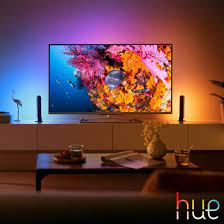
\includegraphics[scale=0.5]{hue.jpg}
    \caption{Philips Hue Center}
    \label{fig::hue:top}
\end{figure}
\begin{figure}[ht]
    \centering
    \begin{minipage}{0.4\textwidth}
        \caption{Philips Hue Over}
        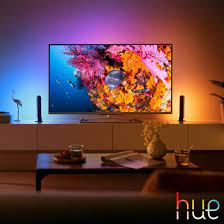
\includegraphics[width=\textwidth]{hue.jpg}
        \label{fig::hue:left}
    \end{minipage}
    \hfill
    \begin{minipage}{0.4\textwidth}
        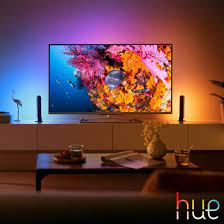
\includegraphics[width=\textwidth]{hue.jpg}
        \caption{Philips Hue Under}
        \label{fig::hue:right}
    \end{minipage}
\end{figure}